% !TEX root = ../main.tex
% chktex-file 21
% chktex-file 46
\section{Spectral Graph Theory}%
\label{sec:sgt}

We start with an introduction to spectral graph theory, which will allow us to characterize and compare the structure of graphs.
Graphs are most commonly described in their vertex base, i.~e.\@ the strength $w_{i j}$ with which pairs $(v_i, v_j)$ of vertices are connected.
\begin{align*}
	G :=&\, (\mathcal{V}, \mathcal{E}, W) \text{ with } W \in \mathbb{R}^{N \times N}, N := |\mathcal{V}|
\end{align*}
In this paper we will only consider undirected graphs with non-negative real weights; thus the adjacency matrix $W$ is positive semi-definite.

The core idea of spectral graph theory essentially is to perform a change of basis and describe graphs in terms of their spectral base instead of their vertex base.
To see what this means, we interpret the adjacency matrix $W$ as a linear operator that operates on so called signals $x \in \mathbb{R}^N$.
A signal $x$ can be interpreted as a function $x: \mathcal{V} \to \mathbb{R}$ that assigns a signal strength to each vertex.
By applying $Wx$ the given signal strengths $x_i$ are shifted according to the connection strenghts $w_{i j}$ to neighboring vertices $v_j$.
This interpretation of graphs is very similar to that of Markov chains where signals represent probability distributions.

\subsection{Relating Graph Signals to Real Functions}%
\label{sec:sgt:real}

Let us now compare discrete graph signals $x: \mathcal{V} \to \mathbb{R}$ to continuous real functions $f: \mathbb{R} \to \mathbb{R}$.
Both only differ in their domain.
The domain $\mathbb{R}$ of $f$ has an inherent structure, the real number line, which provides a strict ordering of its elements and a notion of distance between them.
The domain $\mathcal{V}$ of $x$ however has no such inherent structure, i.~e.\@ $v_1 < v_2$ for two vertices $v_1, v_2$ does not have a clear meaning.
The structure of $\mathcal{V}$ fully depends on the graph $G$ that is acting on it.
Intuitively graph signals can thus be understood as a discretized generalization of real functions, where the underlying structure of the input domain is not fixed but can be freely chosen.
\begin{figure}
	\centering
	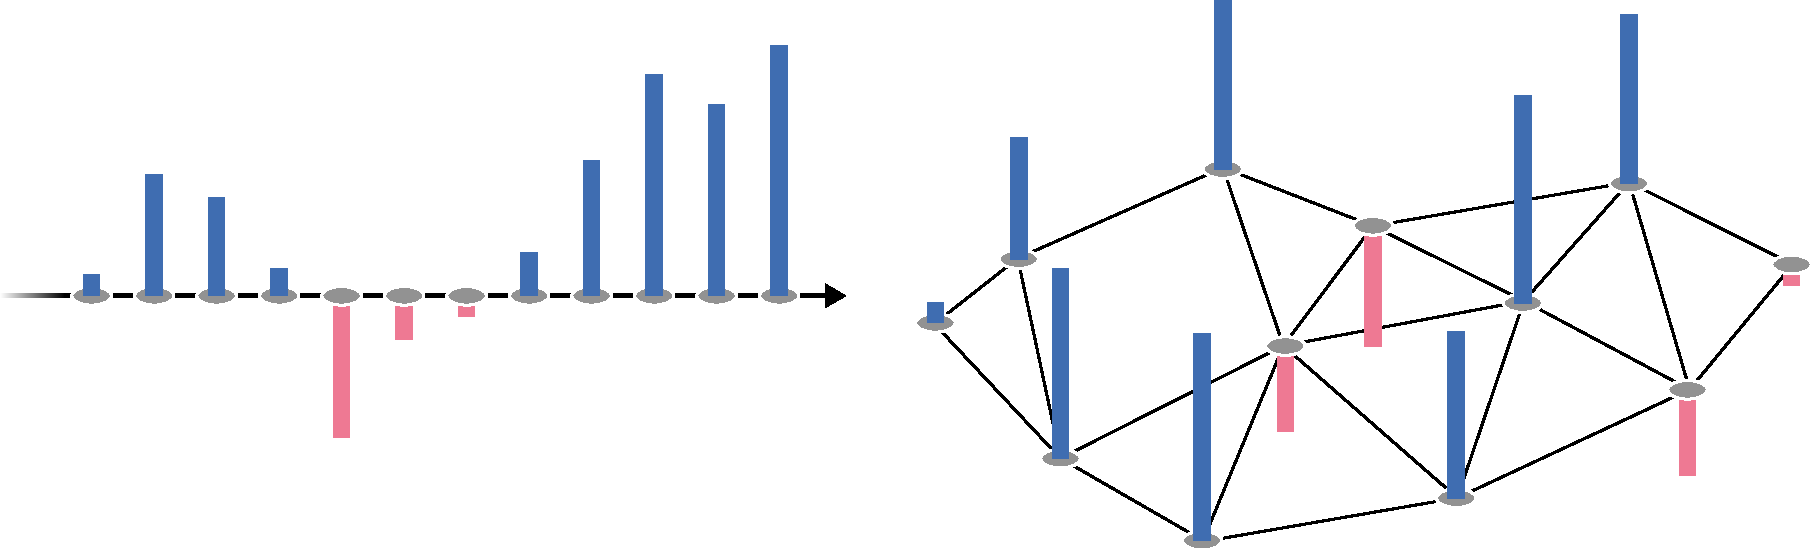
\includegraphics[width=0.9\linewidth]{gfx/sgt/real-graph.pdf}
	\caption{
		Illustration of how the discretized real number line can be interpreted as an infinite linear graph, compared to some arbitrary finite non-linear graph.
		The blue bars show the signal strength at each vertex.
	}\label{fig:sgt:real-graph}
\end{figure}
Figure~\ref{fig:sgt:real-graph} shows that all real functions $f$ can be seen as signals $x$ of the graph described by the real number line\footnote{
	Technically this is not correct, since $\mathbb{R}$ is continuous whereas all vertex sets $\mathcal{V}$ have to be discrete.
	To build an intuition for graph signals, this detail can however be ignored.
}.
Both, real functions and graph signals, can be described as vectors in their time/vertex base:
\begin{equation}
	\begin{split}
		f = \int_{\mathbb{R}} f(t) b_t dt
		\Rightarrow \langle f, b_t \rangle = f(t)
	\end{split}
	\quad\text{and}\quad
	\begin{split}
		x = \sum_{i = 1}^{N} x_i b_i
		\Rightarrow \langle x, b_i \rangle = x_i
	\end{split}
\end{equation}
Here ${\{ b_i \}}_{v_i \in \mathcal{V}}$ denotes the standard basis of the adjacency matrix $W$.
Similarly ${\{ b_t \}}_{t \in \mathbb{R}}$ denotes the infinite dimensional standard basis of the space of real functions, where $\langle \cdot, b_t \rangle := \delta_t(\cdot)$, with $\delta$ denoting the Dirac delta function.

\subsection{Extending the Fourier Transform to Graphs}%
\label{sec:sgt:fourier}

As mentioned at the beginning of this section, the core idea of spectral graph theory is to express graph signal vectors $x$ in the spectral basis ${\{ u_i \}}_{i = 1}^{N}$ instead of the standard vertex basis ${\{ b_i \}}_{v_i \in \mathcal{V}}$.
